\chapter{Target Platform}
\label{vehicle_info}

\begin{figure}[H]
	\centering
	\includegraphics[width=0.6\textwidth]{Images/platform/car.jpg}
	\caption{Model car external view}
	\label{model_car}
\end{figure}

The AutoNOMOS Model Car presented in Figure \ref{model_car} is a 10:1 scaled car, developed as a research platform for educational purposes at Dahlem Center for Machine Learning and Robotics of Freie Universitat Berlin \cite{dcmlr}. An overview of the hardware and software components is presented in the next two sections. 

\section{Hardware Components}
The target platform for validating the planner is a 1:10 scale model car (AutoNOMOS Mini V3) as shown in Figure \ref{model_car}, it is developed as an education and research platform. The car is a modified RC platform, different hardware components used are described in Figure \ref{internalcar}. The main components are a Brushless DC-Servomotor (FAULHABER 2232) to drive and measure speed, a servo motor (HS-645MG) to control the Ackerman steering, IMU (MPU6050) to measure the orientation of the car. The three modules mentioned are controlled with an Arduino Nano which communicates the data to the main CPU (Odroid XU4 - Embedded Computer). Other important components are a depth camera (realsense sr300) for forward vision and perceiving the shape of obstacles ahead, 2D-Lidar (RPLidar), WiFi Dongle, Fisheye Camera for localizing car based on markers on the roof. The Figure \ref{moduleconnections} presents connections across different modules present in the car.
\begin{figure}
	\centering
	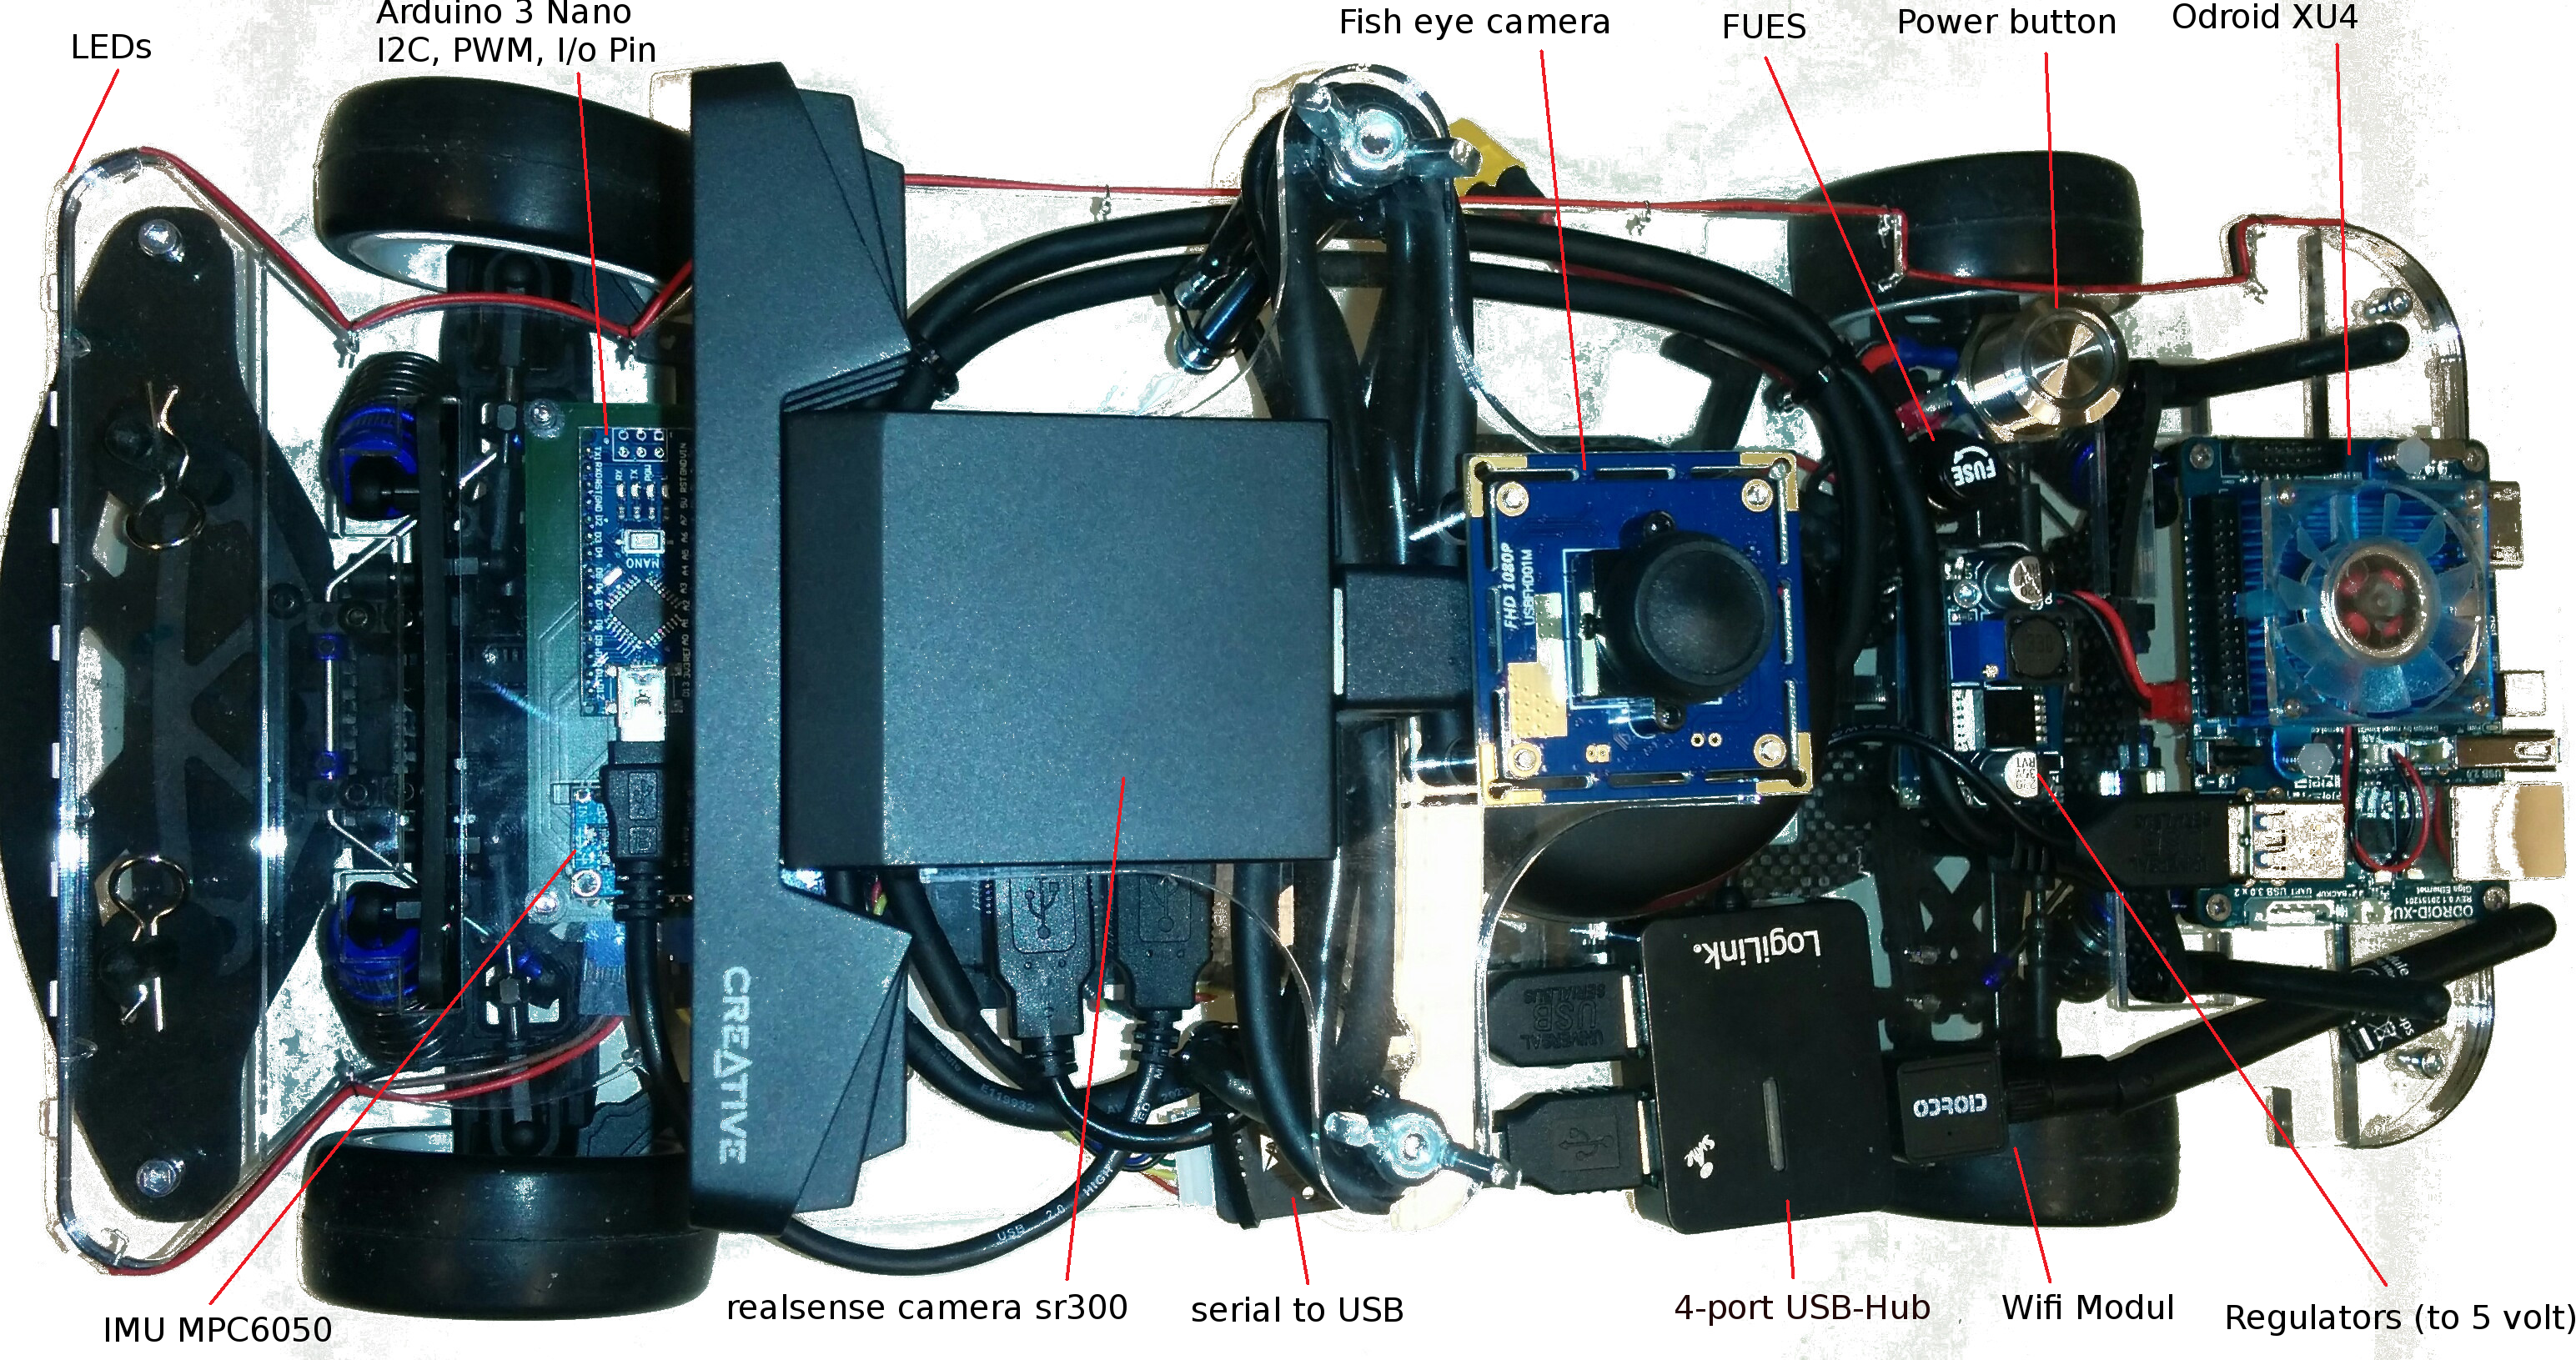
\includegraphics[width=0.8\textwidth]{Images/platform/car_internals.png}
	\caption{Internal components of Model Car \cite{model_car_archi}}
	\label{internalcar}
\end{figure}

\begin{figure}
	\centering
	\includegraphics[width=0.8\textwidth]{Images/platform/hardware_Connections.png}
	\caption{Module Connections \cite{model_car_archi}}
	\label{moduleconnections}
\end{figure}

\section{Software Components}
The CPU onboard runs Robot Operating System (ROS) on top of Ubuntu. ROS is a widely known framework for robotics applications due to its modularity and distributed nature. Modularity allows the application designer to choose which modules to be developed and which modules to be used directly. There are thousands of packages available open-source developed by the community which help to realize a project in a short time. The distributed nature of ROS allows to distribute modules across different platforms based on hardware requirements and communicate easily across them. Though ROS is not real-time capable, it is fast and well suited for robots running in laboratory environments. Many of the issues present in ROS are being addressed in ROS2.0 aiming at industrial scale robots. 

The model car implements core components for motor control, reading data from sensors, Odometry, Camera interfaces etc. There are community developed packages for visual GPS to track markers on the roof and localize car, line detection, traffic sign detection etc.

In summary, the model car features all the components to drive the car autonomously, but there are limitations on the accuracy of measurements, control and computational resources on board. 

%\section{Sensors}
%\section{Architecture \& Computational Power}
%\section{Vehicle Control}
%\section{Localisation}
